\documentclass[tikz,border=15pt]{standalone}
\usetikzlibrary{positioning, arrows.meta, matrix}

\begin{document}
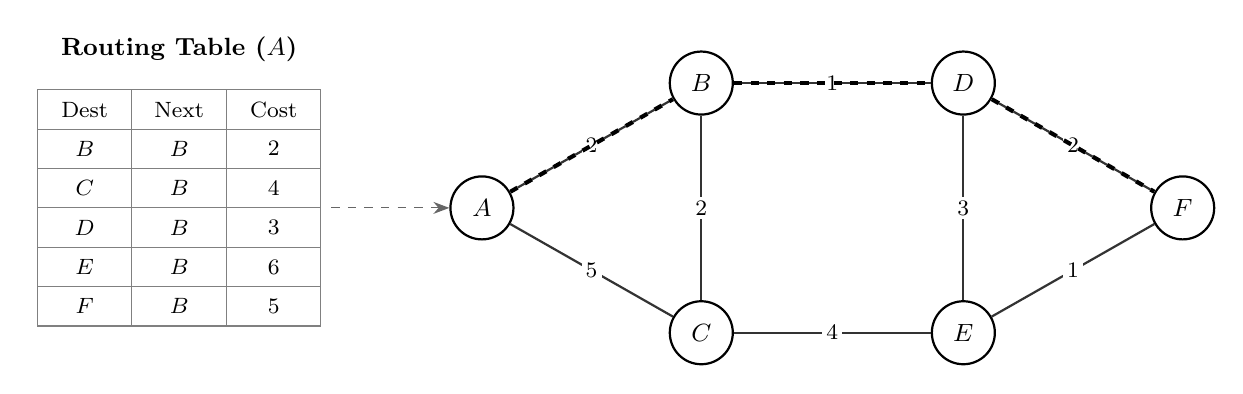
\begin{tikzpicture}[
    >={Stealth[scale=1.2]},
    node distance=2cm and 2.5cm,
    router/.style={circle, draw=black, thick, minimum size=0.8cm, inner sep=0pt, font=\small},
    edge/.style={draw=black!80, thick},
    weight/.style={fill=white, inner sep=1.5pt, font=\footnotesize}
]

% Graph nodes
\node[router] (A) {$A$};
\node[router, above right=1cm and 2.2cm of A] (B) {$B$};
\node[router, below right=1cm and 2.2cm of A] (C) {$C$};
\node[router, right=2.5cm of B] (D) {$D$};
\node[router, right=2.5cm of C] (E) {$E$};
\node[router, below right=1cm and 2.2cm of D] (F) {$F$};

% Graph edges
\draw[edge] (A) -- node[weight] {2} (B);
\draw[edge] (A) -- node[weight] {5} (C);
\draw[edge] (B) -- node[weight] {1} (D);
\draw[edge] (B) -- node[weight] {2} (C);
\draw[edge] (C) -- node[weight] {4} (E);
\draw[edge] (D) -- node[weight] {3} (E);
\draw[edge] (D) -- node[weight] {2} (F);
\draw[edge] (E) -- node[weight] {1} (F);

% Highlighted shortest path (A -> B -> D -> F)
\draw[edge, double=black, double distance=1.5pt, draw=white, dashed] (A) -- (B);
\draw[edge, double=black, double distance=1.5pt, draw=white, dashed] (B) -- (D);
\draw[edge, double=black, double distance=1.5pt, draw=white, dashed] (D) -- (F);

% Routing Table for A
\matrix (table) [
    matrix of nodes,
    nodes={draw=black!50, minimum width=1.2cm, minimum height=0.5cm, anchor=center, font=\footnotesize},
    column sep=-\pgflinewidth,
    row sep=-\pgflinewidth,
    left=1.5cm of A
] {
    Dest & Next & Cost \\
    $B$ & $B$ & 2 \\
    $C$ & $B$ & 4 \\
    $D$ & $B$ & 3 \\
    $E$ & $B$ & 6 \\
    $F$ & $B$ & 5 \\
};
\node[above=0.1cm of table, font=\small\bfseries] {Routing Table ($A$)};

% Pointer from table to node A
\draw[->, dashed, black!60] (table.east) -- (A.west);

\end{tikzpicture}
\end{document}